% ==========================================
% BAB V IMPLEMENTASI
% ==========================================
\cleardoublepage
\chapter{IMPLEMENTASI}
\label{chap:implementasi}

\section{Lingkungan Implementasi}
Bagian ini menjelaskan spesifikasi perangkat keras dan perangkat lunak yang digunakan dalam tahap implementasi penelitian. Implementasi dilakukan pada platform \textit{cloud-based notebook}, yaitu Kaggle Notebook dan Google Colaboratory (Google Colab), sehingga spesifikasi perangkat keras yang digunakan bersifat dinamis dan disediakan secara otomatis oleh masing-masing penyedia layanan.

\subsection{Lingkungan Perangkat Keras}
Spesifikasi sumber daya komputasi yang digunakan pada masing-masing platform selama penelitian ini berlangsung adalah sebagai berikut:
\begin{enumerate}
	\item Kaggle Notebook
	\begin{enumerate}
		\item Prosesor: 4 \textit{vCPU}
		\item Memori (RAM): hingga 29 GB
		\item GPU: NVIDIA Tesla T4 x2 (2 x 16 GB VRAM)
	\end{enumerate}
	\item Google Colaboratory
	\begin{enumerate}
		\item Prosesor: 2 \textit{vCPU}
		\item Memori (RAM): 12--13 GB
		\item GPU: NVIDIA Tesla T4 (16 GB VRAM), digunakan jika tersedia. Saat tidak tersedia, \textit{runtime} dijalankan menggunakan CPU.
	\end{enumerate}
\end{enumerate}

\subsection{Lingkungan Perangkat Lunak}
Perangkat lunak yang digunakan untuk mendukung proses pengembangan adalah:
\begin{enumerate}
	\item Sistem Operasi: Linux (\textit{runtime environment} berbasis Ubuntu yang disediakan oleh Kaggle Notebook dan Google Colab)
	\item Bahasa Pemrograman: Python 3.10+ 
	\item \textit{Platform Notebook}: Kaggle Notebook dan Google Colaboratory (Google Colab)
	\item \textit{Library} Utama: % isi sesuai library yang dipakai
	\item \textit{Driver}: CUDA Toolkit dan cuDNN (terpasang otomatis pada \textit{runtime} GPU Kaggle/Colab)
\end{enumerate}

\section{Pengumpulan Data}

Dataset yang digunakan dalam penelitian ini merupakan dataset citra \textit{CT scan} (\textit{Computed Tomography}) tumor otak yang dikumpulkan dari dua sumber berbeda, menghasilkan total 557 gambar yang terbagi ke dalam tiga kelas, yaitu \textit{no tumor} (otak normal), glioma, dan meningioma. Karakteristik pengumpulan dan pembagian data ini dijabarkan sebagai berikut:

\begin{enumerate}
	\item Sumber Pertama: Platform Radiopaedia (\textit{radiopaedia.org})\\
	Sebuah platform referensi radiologi kolaboratif berbasis komunitas yang memuat ribuan kasus pencitraan medis klinis yang dikontribusikan oleh para radiologis di seluruh dunia. Pengumpulan data dari sumber ini dilakukan melalui teknik \textit{web scraping}, yakni pengambilan gambar secara otomatis dari halaman-halaman kasus \textit{CT scan} otak yang relevan. Citra yang dikumpulkan mencakup tiga kategori: gambar \textit{CT scan} dengan diagnosis glioma, gambar \textit{CT scan} dengan diagnosis meningioma, dan gambar \textit{CT scan} otak normal (\textit{no tumor}). Gambar-gambar dari Radiopaedia memiliki karakteristik klinis yang bervariasi karena berasal dari berbagai institusi dan perangkat pencitraan yang berbeda-beda, sehingga mencerminkan keragaman kondisi akuisisi citra yang realistis.
	
	\item Sumber Kedua: Dataset Publik Mendeley Data\\
	Sumber kedua berasal dari dataset publik yang tersedia di platform Mendeley Data \cite{AlKadi2022Unpaired}. Dataset ini menyediakan 80 gambar citra \textit{CT scan} tumor otak beserta \textit{mask} segmentasi tumornya, yaitu citra biner yang menandai secara piksel wilayah tumor pada setiap gambar. Keberadaan \textit{mask} pada dataset ini memperkaya representasi visual kelas tumor dalam dataset keseluruhan, sekaligus memberikan informasi spasial lokasi tumor yang dapat dimanfaatkan untuk keperluan evaluasi XAI yang digunakan.
	
\end{enumerate}

Gambar-gambar dari kedua sumber tersimpan dalam tiga format file berbeda, yaitu PNG (239 gambar, 42,9\%), JPG (221 gambar, 39,7\%), dan JPEG (97 gambar, 17,4\%), dengan resolusi yang bervariasi mulai dari $205 \times 255$ hingga $1.365 \times 1.365$ piksel. Setelah dilakukan penggabungan dari kedua sumber, dataset dibagi ke dalam tiga subset, yaitu data latih (\textit{train}) sebanyak 386 gambar (69,3\%), data uji (\textit{test}) sebanyak 99 gambar (17,8\%), dan data validasi (\textit{val}) sebanyak 72 gambar (12,9\%). Pembagian dataset ke dalam tiga subset tersebut dilakukan secara stratifikasi berdasarkan kelas, sehingga proporsi setiap kelas (\textit{no tumor}, glioma, dan meningioma) terjaga secara merata di seluruh subset \textit{train}, \textit{val}, dan \textit{test}.

Mengingat gambar-gambar dari sumber kedua (Mendeley Data) memiliki karakteristik yang berbeda dibandingkan sumber pertama, penelitian ini merancang tiga skenario eksperimen \textit{splitting} data Mendeley Data untuk mengevaluasi dampaknya terhadap generalisasi model. Ketiga skenario tersebut adalah sebagai berikut:
\begin{enumerate}
	\item Uji \\
	Data sumber kedua pada subset \textit{test} saja: Seluruh gambar dari sumber kedua ditempatkan pada subset \textit{test}. Skenario ini bertujuan untuk mengukur kemampuan generalisasi model yang dilatih sepenuhnya pada data sumber pertama ketika diuji pada distribusi data yang berbeda.
	\begin{table}[h]
		\centering
		\begin{tabular}{|l|c|c|c|c|}
			\hline
			Kategori            & Tumor & Tanpa Tumor & Total & Persentase (\%) \\
			\hline
			Train (Latih)       & 173 & 73  & 246 & 44.17 \\
			Validation (Validasi) & 75  & 49  & 124 & 22.26 \\
			Test (Uji)          & 145 & 42  & 187 & 33.57 \\
			Total               & 393 & 164 & 557 & 100 \\
			\hline
		\end{tabular}
		\caption{Pembagian Data Skenario 1}
		\label{tab:dataset_test}
	\end{table}
	
	\item Validasi dan Uji \\
	Data sumber kedua pada subset \textit{val} dan \textit{test}: Gambar dari sumber kedua didistribusikan ke dalam subset \textit{val} dan \textit{test}, sementara subset \textit{train} tetap hanya berisi data dari sumber pertama. Skenario ini memungkinkan proses validasi dan pengujian dilakukan pada distribusi yang lebih beragam, sekaligus menjaga proses pelatihan tetap bersih dari data sumber kedua.
	\begin{table}[h]
		\centering
		\begin{tabular}{|l|c|c|c|c|}
			\hline
			Kategori            & Tumor & Tanpa Tumor & Total & Persentase (\%) \\
			\hline
			Train (Latih)       & 173 & 73  & 246 & 44.17 \\
			Validation (Validasi) & 114 & 49  & 163 & 29.26 \\
			Test (Uji)          & 106 & 42  & 148 & 26.57 \\
			Total               & 393 & 164 & 557 & 100 \\
			\hline
		\end{tabular}
		\caption{Pembagian Data Skenario 2}
		\label{tab:dataset_val_test}
	\end{table}
	
	\item Validasi, Uji, dan Latih \\
	Data sumber kedua pada seluruh subset (\textit{train}, \textit{val}, dan \textit{test}): Gambar dari sumber kedua didistribusikan secara proporsional ke seluruh subset \textit{train}, \textit{val}, dan \textit{test}. Skenario ini mencerminkan kondisi pelatihan yang memanfaatkan keseluruhan data yang tersedia dari kedua sumber secara terpadu.
	\begin{table}[h]
		\centering
		\begin{tabular}{|l|c|c|c|c|}
			\hline
			Kategori   & Tumor & Tanpa Tumor & Total & Persentase (\%) \\
			\hline
			Train      & 224 & 73  & 297 & 53.32 \\
			Validation & 90  & 49  & 139 & 24.96 \\
			Test       & 79  & 42  & 121 & 21.72 \\
			Total      & 393 & 164 & 557 & 100 \\
			\hline
		\end{tabular}
		\caption{Pembagian Data Skenario }
		\label{tab:dataset_all}
	\end{table}
	
\end{enumerate}
Ketiga skenario ini dirancang untuk mengkaji sejauh mana asal-usul dan penempatan data sumber kedua memengaruhi kinerja model klasifikasi, khususnya dalam konteks perbedaan distribusi (\textit{domain shift}) antara kedua sumber data. Kondisi dataset mentah yang heterogen ini menjadi dasar dilakukannya proses \textit{preprocessing}.

\section{Pemrosesan Data}

\subsection{Pemrosesan Umum}
Proses \textit{preprocessing} dilakukan untuk menyeragamkan seluruh gambar agar memenuhi standar \textit{input} model jaringan saraf tiruan yang digunakan. Terdapat tiga tahap \textit{preprocessing} yang diterapkan pada keseluruhan 557 gambar dataset:

\begin{enumerate}
	\item Konversi Format\\
	Seluruh gambar dikonversi ke format PNG untuk memastikan konsistensi format file. Sebelum \textit{preprocessing}, terdapat 318 gambar (57,1\%) yang bukan berekstensi PNG. Setelah \textit{preprocessing}, keseluruhan 557 gambar tersimpan dalam format PNG.
\end{enumerate}

Hasil akhir proses \textit{preprocessing} menunjukkan perbaikan yang menyeluruh pada seluruh aspek yang disasar. Ukuran rata-rata file juga berkurang secara signifikan dari 96,52 KB menjadi 30,86 KB per gambar, dengan total ukuran dataset menyusut dari 52,5 MB menjadi 16,79 MB --- penghematan sekitar 68\% ruang penyimpanan. 

Distribusi rata-rata intensitas piksel antarsplit pun relatif konsisten, dengan nilai \textit{test} sebesar 53,47, \textit{train} sebesar 58,56, dan \textit{val} sebesar 64,16 (skala 0--255), yang mengindikasikan tidak adanya bias kecerahan yang signifikan antar subset data. Ringkasan perbandingan kondisi dataset sebelum dan sesudah \textit{preprocessing} disajikan pada Tabel~\ref{tab:preprocessing}.

\begin{table}[htbp]
	\centering
	\caption{Perbandingan Kondisi Dataset Sebelum dan Sesudah \textit{Preprocessing}}
	\label{tab:preprocessing}
	\begin{tabular}{|l|l|l|}
		\hline
		\textbf{Aspek} & \textbf{Sebelum} & \textbf{Setelah} \\ \hline
		Mode warna & RGB, L, RGBA, P (4 varian) & RGB \\ \hline
		Resolusi & 15 varian berbeda & $224 \times 224$ \\ \hline
		Format file & PNG, JPG, JPEG & PNG \\ \hline
		Ukuran file rata-rata & 96,52 KB & 30,86 KB \\ \hline
		Total ukuran dataset & 52,5 MB & 16,79 MB \\ \hline
	\end{tabular}
\end{table}

\subsection{Pemrosesan Eksperimen}
\subsubsection{Gaussian Denoise dan CLAHE}
Berdasarkan hasil analisis statistik, terdapat perbedaan yang terukur antara dataset sebelum dan sesudah diterapkan \textit{preprocessing} Gaussian dan CLAHE, sebagaimana ditunjukkan pada Tabel~\ref{tab:analisis_statistik}.

\begin{table}[htbp]
	\centering
	\caption{Perbandingan Parameter Dataset Sebelum dan Sesudah \textit{Preprocessing}}
	\label{tab:analisis_statistik}
	\begin{tabular}{|l|c|c|l|}
		\hline
		\textbf{Parameter} & \textbf{Sebelum} & \textbf{Sesudah} & \textbf{Perubahan} \\ \hline
		Intensitas minimum & 0,0 & 3,78--3,93 & +3,78--3,93\\ \hline
		Rata-rata intensitas (\textit{train}) & 58,56 & 64,41 & +5,85 \\ \hline
		Rata-rata intensitas (\textit{val}) & 64,16 & 69,79 & +5,63 \\ \hline
		Rata-rata intensitas (\textit{test}) & 53,47 & 59,68 & +6,21 \\ \hline
		Standar deviasi (\textit{train}) & 78,45 & 77,81 & -0.64 \\ \hline
		Ukuran file rata-rata & 30,86 KB & 52,32 KB & +69,6\% \\ \hline
	\end{tabular}
\end{table}

Pergeseran nilai intensitas minimum dari 0,0 menjadi 3,78-3,93 menunjukkan bahwa Gaussian berhasil menghilangkan piksel terisolasi bernilai nol yang merepresentasikan \textit{noise} impulsif pada citra \textit{CT scan}. Kenaikan rata-rata intensitas sebesar 5,6--6,2 poin secara konsisten di seluruh subset menunjukkan bahwa CLAHE berhasil meningkatkan kontras lokal citra. Selain itu, standar deviasi yang tidak meningkat melainkan sedikit menurun mengindikasikan bahwa peningkatan kontras berlangsung terkontrol tanpa \textit{over-amplification noise}. Hal ini sejalan dengan pernyataan \textcite{putra2025enhanced} bahwa \textit{Gaussian filtering} berfungsi untuk meredam \textit{noise} frekuensi tinggi, sedangkan CLAHE bertujuan meningkatkan kontras lokal tanpa memperkuat \textit{noise} pada citra medis.

\subsubsection{Wavelet Denoise dan Intensity Normalization}


\section{Implementasi Arsitektur Model}

\subsection{Correlation Learning Mechanism (CLM)}

Berdasarkan diagram alur eksperimen, komponen ANN yang disorot dengan warna biru mengalami penyesuaian melalui \textit{hyperparameter tuning}, meliputi:
\begin{itemize}
	\item Dropout Rate: Penambahan \textit{dropout} pada setiap \textit{hidden layer} ANN, diuji pada nilai 0,05; 0,10; dan 0,20 untuk mencegah \textit{overfitting} akibat keterbatasan sampel CT Scan. Nilai terlalu kecil kurang efektif meregularisasi, sedangkan terlalu besar berisiko \textit{underfitting}.
	\item Jumlah Iterasi: Penyesuaian total iterasi pelatihan BPTA pada nilai 3.000, 5.000, dan 10.000. Iterasi terlalu sedikit membuat bobot belum konvergen, sedangkan terlalu banyak meningkatkan waktu pelatihan dan risiko \textit{overfitting}.
	\item Learning Rate BPTA: Penyesuaian laju pembelajaran \textit{gradient descent} klasik pada nilai 0,0001; 0,001; dan 0,01. Nilai terlalu kecil membuat konvergensi lambat, sedangkan terlalu besar berisiko \textit{overshooting} karena BPTA tidak memiliki mekanisme adaptif.
\end{itemize}

Ketiga parameter diuji bersamaan melalui \textit{grid search} (3×3×3 = 27 kombinasi), dan kombinasi terbaik dipilih berdasarkan \textit{composite score} dari lima metrik evaluasi (\textit{accuracy, precision, recall, specificity}, F1), bukan akurasi semata, agar hasil lebih representatif terhadap generalisasi model.

\begin{table}[htbp]
	\centering
	\caption{Best Model setiap Eksperimen CLM}
	\label{tab:best_model_clm}
	\resizebox{\textwidth}{!}{
		\begin{tabular}{|l|c|c|c|c|c|l|}
			\hline
			\textbf{Eksperimen} & \textbf{Acc (\%)} & \textbf{Precision (\%)} & \textbf{Recall (\%)} & \textbf{Specificity (\%)} & \textbf{F1 (\%)} & \textbf{Config Terbaik} \\ \hline
			No Prep / All & 65.3 & 65.3 & 100.0 & 0.0 & 79.0 & LR=0.0001, drop=0.1, iter=5000 \\ \hline
			No Prep / Test & 77.5 & 77.5 & 100.0 & 0.0 & 87.4 & LR=0.00025, drop=0.1, iter=5000 \\ \hline
			No Prep / Val+Test & 71.6 & 71.6 & 100.0 & 0.0 & 83.5 & LR=0.00025, drop=0.1, iter=5000 \\ \hline
			GC / All & 62.8 & 64.4 & 96.2 & 0.0 & 77.2 & LR=0.00025, drop=0.05, iter=5000 \\ \hline
			GC / Test & 77.5 & 77.5 & 100.0 & 0.0 & 87.4 & LR=0.001, drop=0.1, iter=5000 \\ \hline
			GC / Val+Test & 71.6 & 71.6 & 100.0 & 0.0 & 83.5 & LR=0.001, drop=0.1, iter=5000 \\ \hline
			\textbf{WN / All} & \textbf{54.6} & \textbf{61.1} & \textbf{83.5} & \textbf{0.0} & \textbf{70.6} & \textbf{LR=0.00025, drop=0.1, iter=5000} \\ \hline
			WN / Test & 78.6 & 78.4 & 100.0 & 4.8 & 87.9 & LR=0.00025, drop=0.1, iter=5000 \\ \hline
			WN / Val+Test & 73.0 & 72.6 & 100.0 & 4.8 & 84.1 & LR=0.00025, drop=0.1, iter=5000 \\ \hline
		\end{tabular}%
	}
\end{table}

\subsection{Explainable CNN}

Berdasarkan diagram alur eksperimen, terdapat komponen-komponen yang disesuaikan pada tugas akhir ini disorot dengan warna biru, meliputi:
\begin{itemize}
	\item CT Scan Input: Modifikasi fokus modalitas medis utama dari citra MRI menjadi CT Scan. Perubahan ini dilakukan untuk menyessuaikan tujuan utama penelitian untuk menciptakan model pendeteksian otak menggunakan citra medis CT Scan.
	\item Dropout Layer: Penambahan lapisan \textit{Dropout}  setelah proses \textit{Flattening}. Berdasarkan riset Wojciuk dkk. (2024),  \textit{dropout} efektif dalam mencegah masalah \textit{overfitting} pada model pembelajaran mendalam yang memiliki dataset medis dengan distribusi atau kuantitas sampel yang terbatas.
	\item Dense 2 Class: Menyesuaikan ujung struktur model dari keluaran multi-kelas menjadi klasifikasi biner. Modifikasi pada \textit{Dense layer} dan \textit{Output} klasifikasi biner ini merupakan bentuk penyesuaian terhadap spesifikasi dan tujuan dari penelitian ini.
\end{itemize}

\begin{figure}[h]
\centering
\captionsetup{justification=centering}
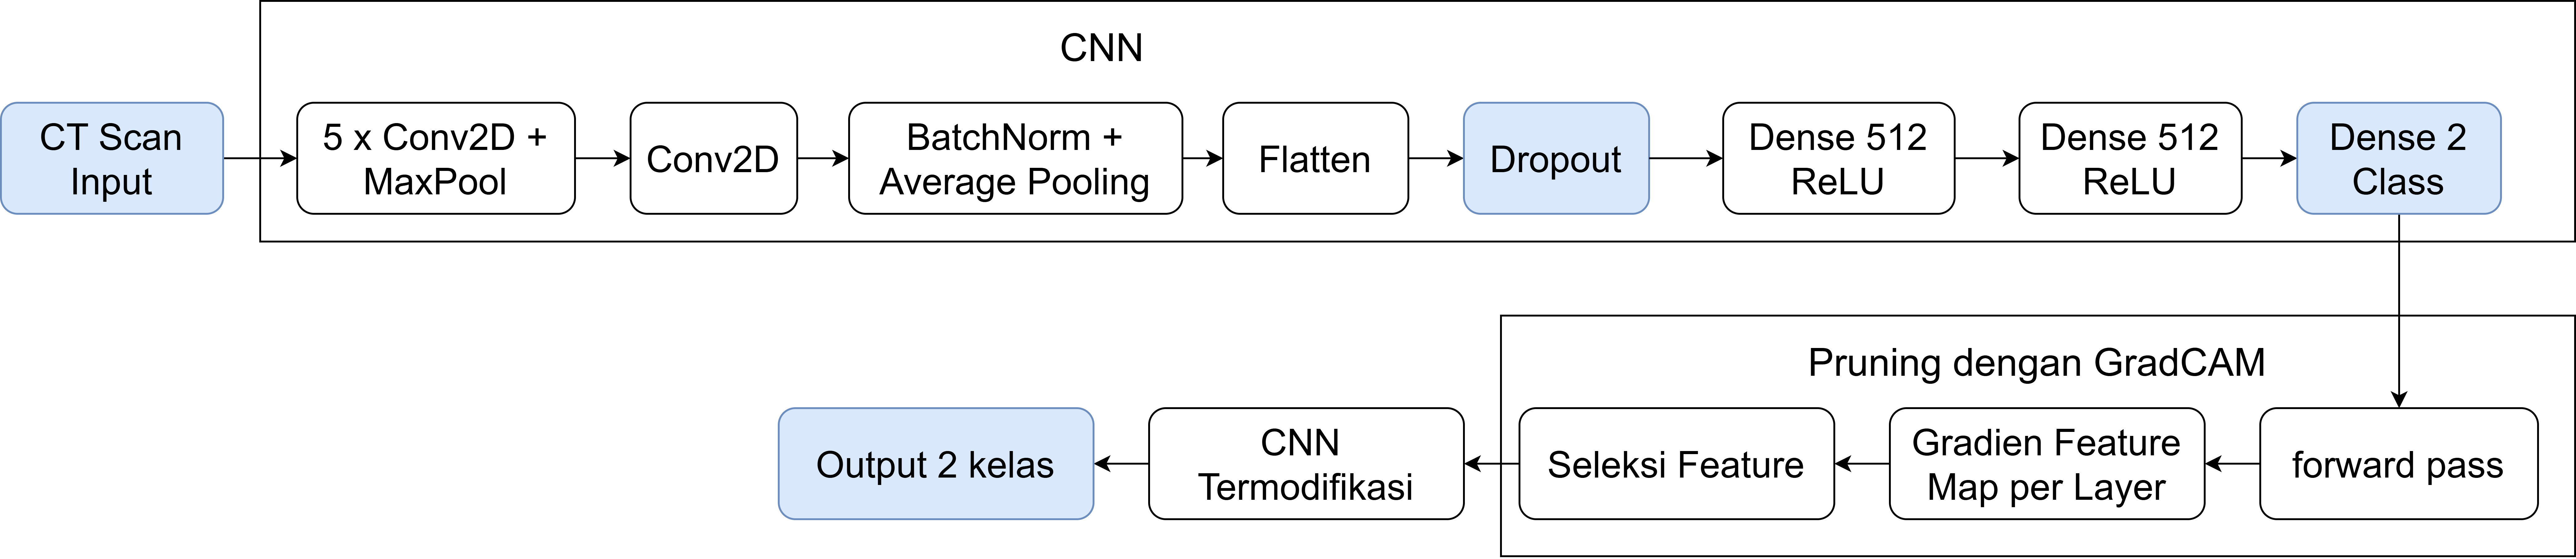
\includegraphics[width=0.85\textwidth]{images/after exp cnn.png}
\caption{Arsitektur Model CNN + ANN}
\label{gambar:afterexpcnn}
\end{figure}

\begin{table}[htbp]
	\centering
	\caption{Best Model setiap Eksperimen Explainable CNN}
	\label{tab:best_model_explainable_cnn}
	\resizebox{\textwidth}{!}{%
		\begin{tabular}{|l|c|c|c|c|c|l|}
			\hline
			\textbf{Eksperimen} & \textbf{Acc (\%)} & \textbf{Precision (\%)} & \textbf{Recall (\%)} & \textbf{Specificity (\%)} & \textbf{F1 (\%)} & \textbf{Config terbaik} \\ \hline
			\textbf{all} & \textbf{70.37} & \textbf{69.64} & \textbf{70.37} & \textbf{47.62} & \textbf{69.94} & \textbf{lr=0.01, bs=64, dr=0.1} \\ \hline
			test & 84.27 & 71.01 & 84.27 & 0.00 & 77.08 & lr=0.0001, bs=40, dr=0.1 \\ \hline
			val+test & 80.95 & 79.94 & 80.95 & 21.43 & 76.54 & lr=0.01, bs=40, dr=0.1 \\ \hline
			GC -- All & 79.26 & 79.89 & 79.26 & 71.43 & 79.50 & lr=0.001, bs=16, dr=0.1 \\ \hline
			\textbf{GC -- Test} & \textbf{71.54} & \textbf{85.43} & \textbf{71.54} & \textbf{80.95} & \textbf{75.28} & \textbf{lr=0.01, bs=64, dr=0.2} \\ \hline
			GC -- Val+Test & 65.08 & 78.16 & 65.08 & 76.19 & 68.02 & lr=0.01, bs=64, dr=0.2 \\ \hline
			WN -- All & 67.41 & 75.52 & 67.41 & 80.95 & 68.59 & lr=0.01, bs=40, dr=0.3 \\ \hline
			WN -- Test & 78.28 & 81.50 & 78.28 & 50.00 & 79.61 & lr=0.0001, bs=40, dr=0.1 \\ \hline
			\textbf{WN -- Val+Test} & \textbf{87.83} & \textbf{88.45} & \textbf{87.83} & \textbf{78.57} & \textbf{88.07} & \textbf{lr=0.0001, bs=40, dr=0.1} \\ \hline
		\end{tabular}%
	}
\end{table}

\subsection{EfficientNetB0}

\begin{figure}[h]
	\centering
	\captionsetup{justification=centering}
	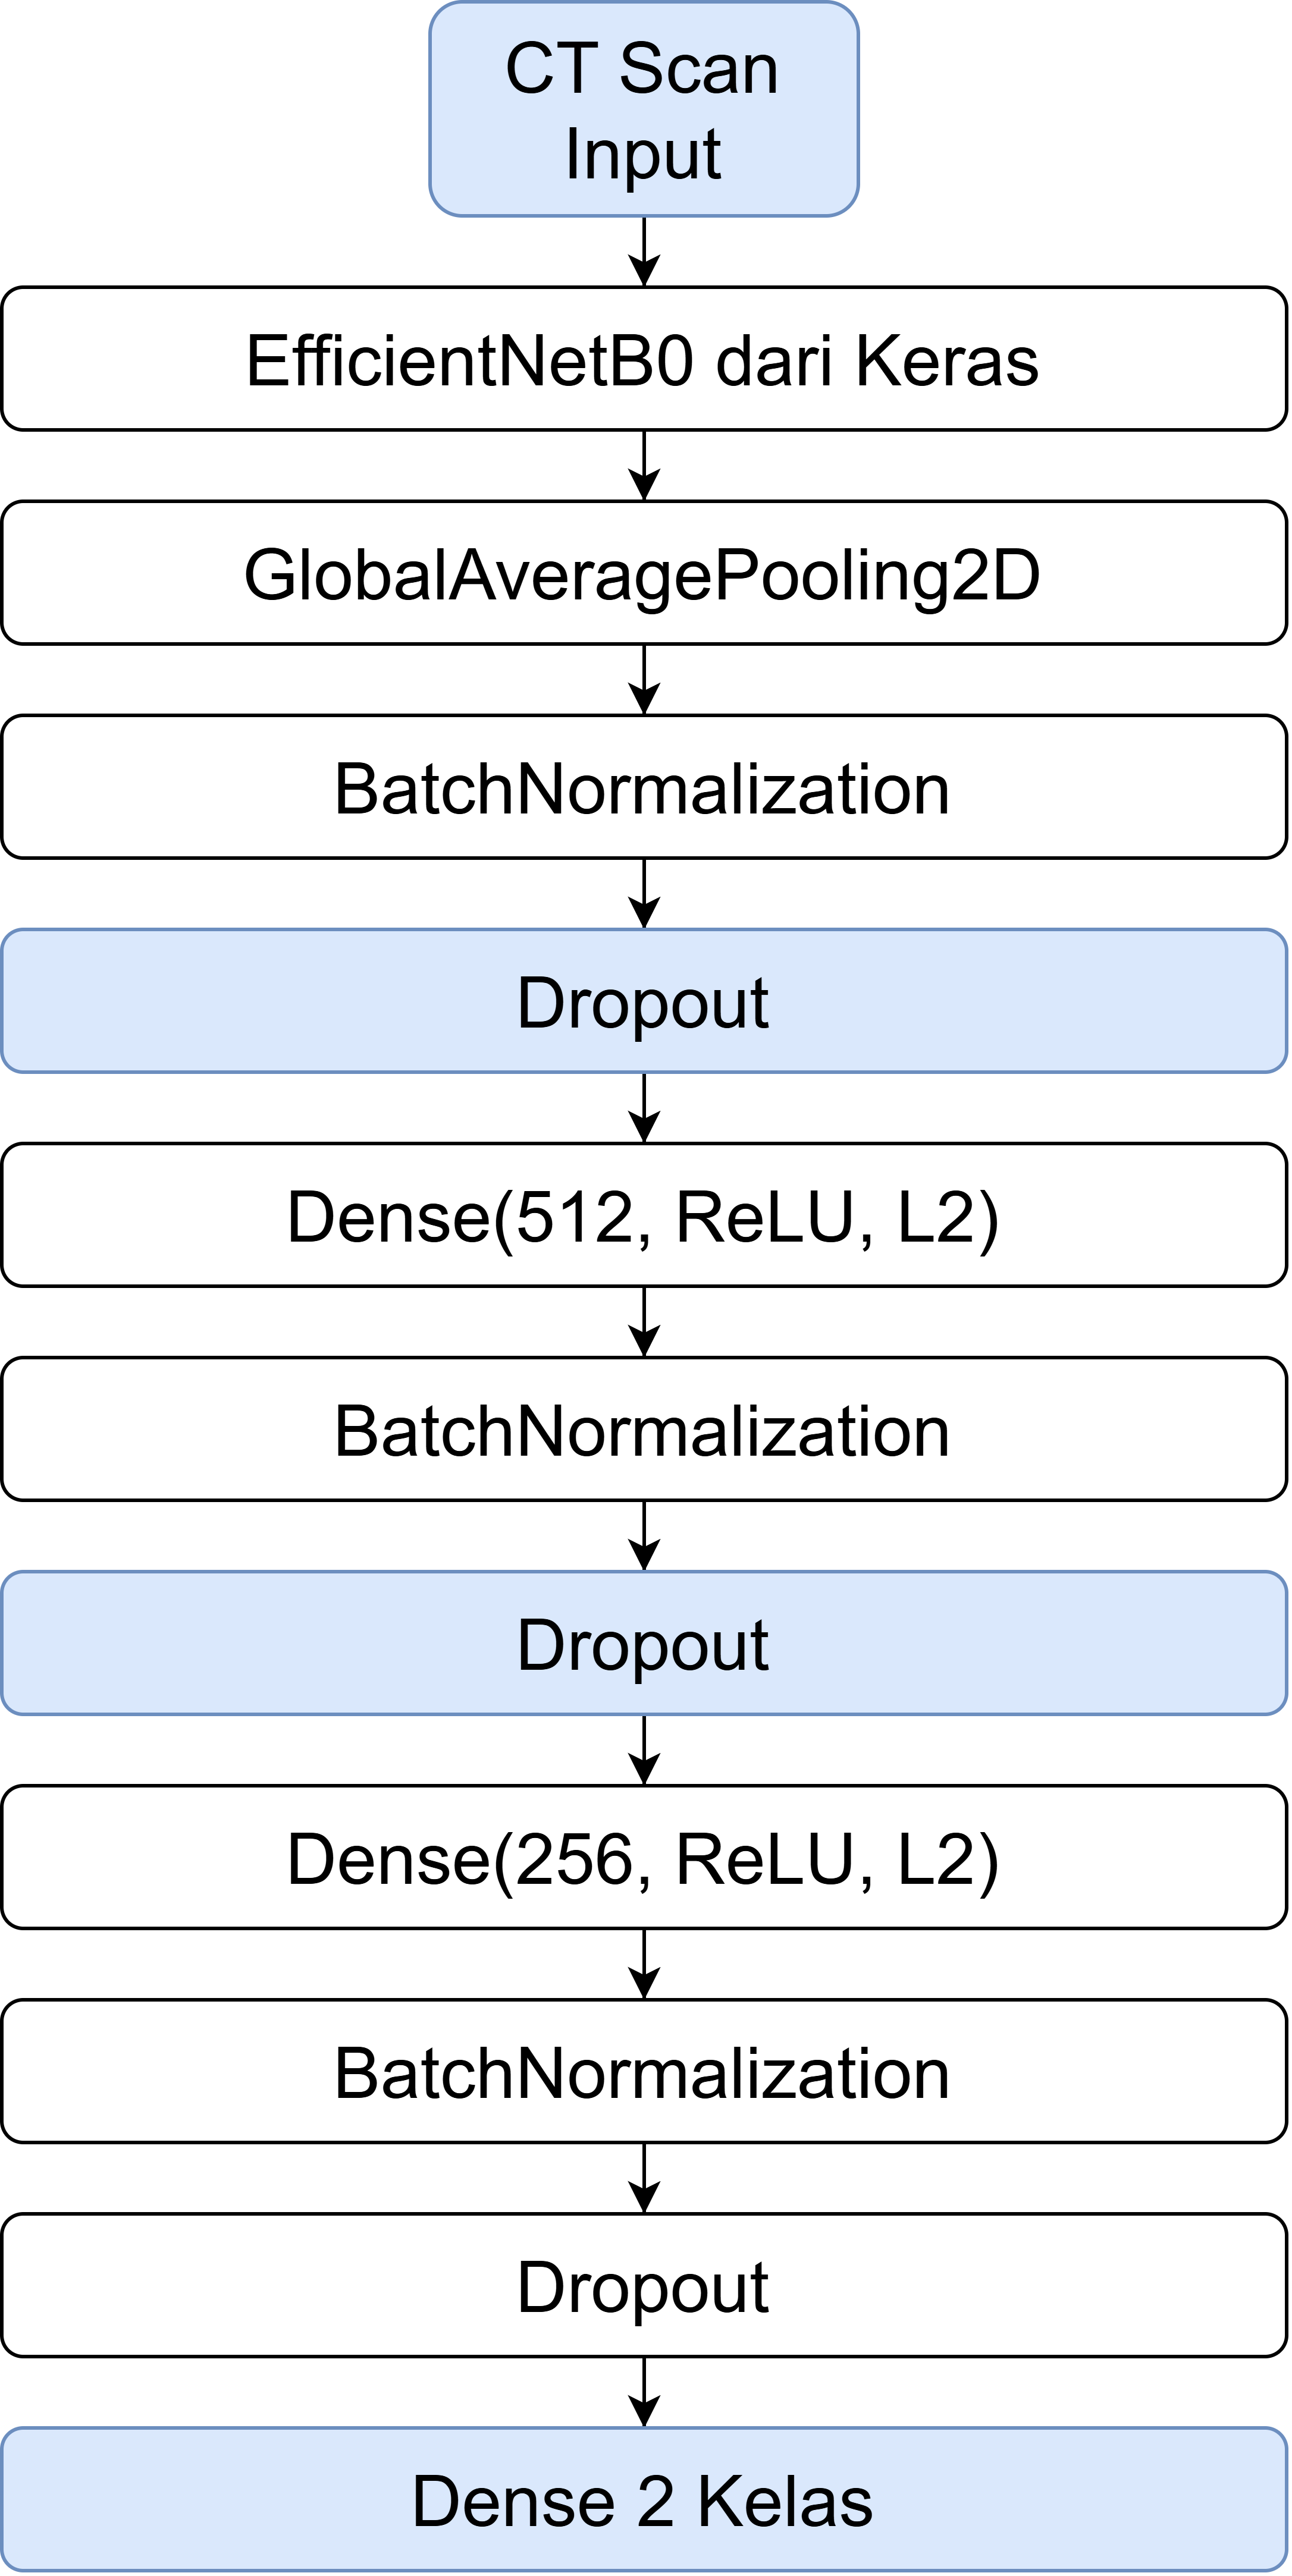
\includegraphics[width=0.5\textwidth]{images/after tl.png}
	\caption{Arsitektur Model EfficientNetB0}
	\label{gambar:aftertransferlearning}
\end{figure}

Berdasarkan diagram alur eksperimen, terdapat komponen-komponen yang disesuaikan pada tugas akhir ini disorot dengan warna biru, meliputi:
\begin{itemize}
	\item CT Scan Input: Modifikasi fokus modalitas medis utama dari citra MRI menjadi CT Scan. Perubahan ini dilakukan untuk menyesuaikan tujuan utama penelitian untuk menciptakan model pendeteksian otak menggunakan citra medis CT Scan.
	\item Dropout Layer: Penambahan lapisan \textit{Dropout} setelah lapisan \textit{BatchNormalization} pertama, yaitu sebelum blok \textit{Dense}(512, ReLU, L2) pada arsitektur model. Berdasarkan riset Wojciuk dkk. (2024), \textit{dropout} efektif dalam mencegah masalah \textit{overfitting} pada model pembelajaran mendalam yang memiliki dataset medis dengan distribusi atau kuantitas sampel yang terbatas.
	\item Dense 2 Class: Menyesuaikan ujung struktur model dari keluaran multi-kelas (4 kelas) menjadi klasifikasi biner (2 kelas). Modifikasi pada \textit{Dense layer} dan \textit{output} klasifikasi biner ini merupakan bentuk penyesuaian terhadap spesifikasi dan tujuan dari penelitian ini, yaitu membedakan citra CT Scan otak normal dan tidak normal (atau sesuai dua kelas target penelitian).
\end{itemize}

\begin{table}[htbp]
	\centering
	\caption{Best Model setiap Eksperimen EfficientNetB0}
	\label{tab:best_model_efficientnetb0}
	\resizebox{\textwidth}{!}{
		\begin{tabular}{|l|c|c|c|c|c|l|}
			\hline
			\textbf{Eksperimen} & \textbf{Acc (\%)} & \textbf{Precision (\%)} & \textbf{Recall (\%)} & \textbf{Specificity (\%)} & \textbf{F1 (\%)} & \textbf{Config terbaik} \\ \hline
			all & 95.56 & 95.63 & 95.56 & 88.10 & 95.49 & lr=0.01, bs=16, dr=0.1 \\ \hline
			test & 93.26 & 94.44 & 93.26 & 92.86 & 93.59 & lr=0.01, bs=16, dr=0.3 \\ \hline
			val+test & 95.24 & 95.42 & 95.24 & 92.86 & 95.30 & lr=0.01, bs=16, dr=0.3 \\ \hline
			GC -- All & 88.89 & 90.69 & 88.89 & 95.24 & 89.18 & lr=0.0001, bs=64, dr=0.1 \\ \hline
			\textbf{GC -- Test} & \textbf{96.63} & \textbf{96.76} & \textbf{96.63} & \textbf{92.86} & \textbf{96.68} & \textbf{lr=0.01, bs=64, dr=0.3} \\ \hline
			GC -- Val+Test & 90.48 & 92.10 & 90.48 & 92.86 & 90.87 & lr=0.01, bs=64, dr=0.2 \\ \hline
			WN -- All & 93.33 & 93.56 & 93.33 & 92.86 & 93.39 & lr=0.01, bs=16, dr=0.1 \\ \hline
			WN -- Test & 93.63 & 94.43 & 93.63 & 90.48 & 93.88 & lr=0.01, bs=40, dr=0.1 \\ \hline
			WN -- Val+Test & 90.48 & 92.89 & 90.48 & 97.62 & 90.96 & lr=0.01, bs=16, dr=0.2 \\ \hline
		\end{tabular}%
	}
\end{table}

\section{\textit{Explainable AI} (Grad-CAM)}

\subsection{GradCAM++ untuk Explainable CNN}

\subsection{GradCAM untuk Transfer Learning EfficientB0}